\chapter{Modelo de Seguridad de iOS}
iOS es un sistema operativo móvil de la multinacional Apple Inc. diseñado para ser
seguro \cite{asg}. Cada dispositivo combina hardware, software y servicios, diseñados para trabajar
conjuntamente para proveer seguridad y al mismo tiempo, que la misma sea transparente para el
usuario.
\begin{figure}[htbp]
    \centering
    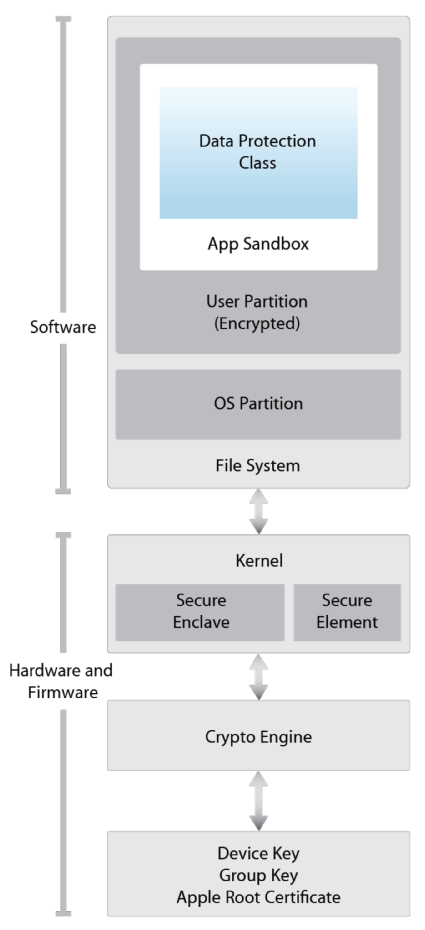
\includegraphics[width=0.3\linewidth]{chapter2/ios_security_architecture}
    \caption{Modelo de seguridad de iOS \cite{asg}.} 
    \label{fig:ch02:security-architecture}
\end{figure}
Características como encriptación del sistema de archivos, asegurar un arranque seguro, asegurar
\textit{KeyChain Data}, vienen habilitadas por defecto. Como se puede observar en la figura \ref{fig:ch02:security-architecture}, la seguridad se extiende más allá del dispositivo, generando un ecosistema seguro.\\
A lo largo de este capítulo se realizara una descripción de los principales aspectos del modelo de seguridad de iOS, basándose en la versión 9.3, lanzada en 2015.
\section{Protección de los datos} \label{fig:ch02:data-protection}
iOS tiene una protección especial para los archivos y los datos personales, la cual sigue intacta inclusive si algunas otras partes del sistema de seguridad fueron comprometidas \cite{asg}. La protección de los datos es implementada construyendo varias claves criptográficas y generando con ellas una jerarquía.\\
Las claves UID y GID\footnote{\textit{Group ID}, por sus siglas en inglés} son AES-256, y fueron integradas al \textit{Secure Enclave} al momento de fabricación del dispositivo. Ningún firmware ni software pueden leerlas directamente, solamente las usa el \textit{Secure Enclave}.\\
Además de UID y GID, existen otras claves criptográficas, las cuales son generadas por el RNG (\textit{Random Number Generator}, por sus siglas en inglés), usando un algoritmo basado en CTR-DRBG. La entropía es generada por la variación del tiempo transcurrido a partir del booteo \cite{asg}. Todo esto ocurre por hardware dentro del \textit{Secure Enclave}.\\
Cada vez que se crea un archivo en la partición de datos, el componente \textit{Data Protection} crea una clave AES-256 para ése archivo (distinta para cada archivo) y se la pasa a \textit{Secure Enclave} para que encripte al archivo con dicha clave. Luego, ésa clave se empaqueta con una (o varias) de las claves de clases, dependiendo de la accesibilidad que va a tener el archivo\footnote{Todos los empaquetamientos se realizan utilizando NIST AES \textit{key wrapping}, según RFC3394 \cite{asg}.}.
Cuando se abre un archivo, su metadata es desempaquetada con la clave del sistema de archivos, revelando la clave particular del archivo y las clases que lo protegen. Se vuelve a desepaquetar, esta vez, con las claves de las clases, para finalmente desencriptar al archivo con su clave única. Este proceso se observa en la Figura \ref{fig:ch02:dataProtection}.
\begin{figure}[hbtp]
    \centering
    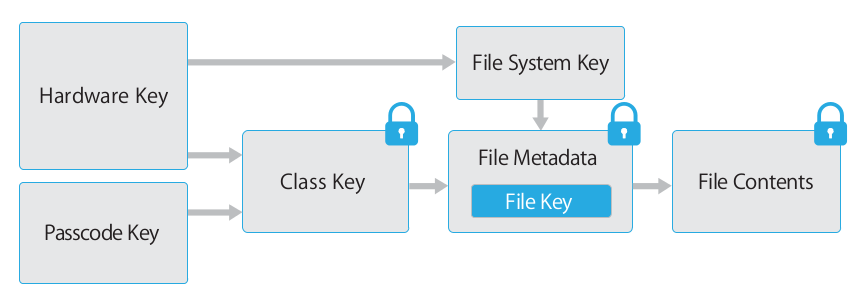
\includegraphics[width=.7\linewidth]{chapter2/ios_fileDataProtection_architecture}
    \caption{Proceso para desempaquetar un archivo \cite{asg}.}
    \label{fig:ch02:dataProtection}
\end{figure}
\section{Código de desbloqueo y Almacenamiento seguro de claves}
iOS soporta un código de desbloqueo de longitud 4 o superior, salvo que el dispositivo tenga un lector de huellas; en ese \'ultimo caso deber\'a contar con al menos 6 d\'igitos. Además de desbloquear el dispositivo, el código provee entropía a ciertas claves de encriptación del sistema, especialmente a las que se encuentran en el componente \textit{Data Protection}. El hecho de que esté muy ligado con el UID\footnote{Id del usuario, explicada en la secci\'on \ref{fig:ch02:arranque}.}, añade una seguridad extra: no se puede intentar quebrar dicho código fuera del dispositivo. Sumado a esto, se le agrega un gran retraso entre intentos fallidos, el cual intenta reducir la cantidad de intentos de un ataque por fuerza bruta. Los retrasos estan calibrados suponiendo que la frecuencia entre un ataque y otro es de 80 milisegundos \cite{asg}.\\
Otra herramienta importante del modelo de seguridad es el almacen de claves llamado Llavero\footnote{Traduccion del termino \textit{keyChain}.}, cuya funcionalidad es proteger las contraseñas y otros datos sensibles de algunas aplicaciones que manejan credenciales propias. Est\'a implementada como una base de datos SQLite \cite{asg}, almacenada en el sistema de archivos. Es única por dispositivo y sólo puede ser accedida mediante el demonio de seguridad, el cual es el encargado de decidir quiénes pueden acceder a los items del \textit{Llavero}. Dicho acceso depende de los siguientes permisos:
\begin{itemize}
\item \emph{Clase del \textit{Llavero}:} Permite asociar un item con su funcionalidad. En el Cuadro \ref{tab:ch02:keychain-classes} se observan las distintas clases provistas por el sistema.
\item \emph{Id de la aplicacion:} Restringe al item para utilizarlo solamente con una aplicaci\'on.
\item \emph{Id del grupo de la aplicacion:} Retringe al item para utilizarlo entre aplicaciones que compartan un GID\footnote{Id del grupo, explicada en la secci\'on \ref{fig:ch02:data-protection}.}. Permite a que un desarrollador comparta credenciales entre sus distintas aplicaciones.
\end{itemize}
\begin{table}[hbtp]
    \centering
    \begin{tabular}{l l}
\textbf{Habilidad}    &    \textbf{Clase}   \\ \hline
Cuando est\'a desbloqueado    &   \textit{kSecAttrAccessibleWhenUnlocked} \\
Despu\'es del primer desbloqueo    &    \textit{kSecAttrAccessibleAfterFirstUnlock} \\
Siempre    &   \textit{kSecAttrAccessibleAlways}    \\
C\'odigo de desbloqueo v\'alido    &    \textit{kSecAttrAccessible} o \textit{WhenPasscodeSetThisDeviceOnly}
    \end{tabular}
    \caption{Clases del \textit{Llavero} seg\'un su funcionalidad \cite{asg}.}
    \label{tab:ch02:keychain-classes}
\end{table}
\section{Seguridad en las aplicaciones}
\subsection{Entorno seguro}
Las aplicaciones son un punto crítico en la seguridad de un dispositivo móvil. iOS provee varias capas de seguridad para las aplicaciones, asegurando que las mismas estén certificadas y verificadas antes de estar disponibles en la tienda \cite{asg}.\\
Todas las aplicaciones de terceros\footnote{\textit{third-party apps}} son aisladas mediante \textit{sandboxing}: tienen denegado el acceso de archivos guardados por otras aplicaciones; tampoco pueden realizar cambios en el dispositivo. En la Figura \ref{fig:ch02:sandboxing} se puede observar lo mencionado anteriormente: cada aplicaci\'on tiene su directorio \textit{Home} para sus archivos, el cual es otorgado aleatoreamente al momento de instalaci\'on.\\
\begin{figure}[hbtp]
	\centering
	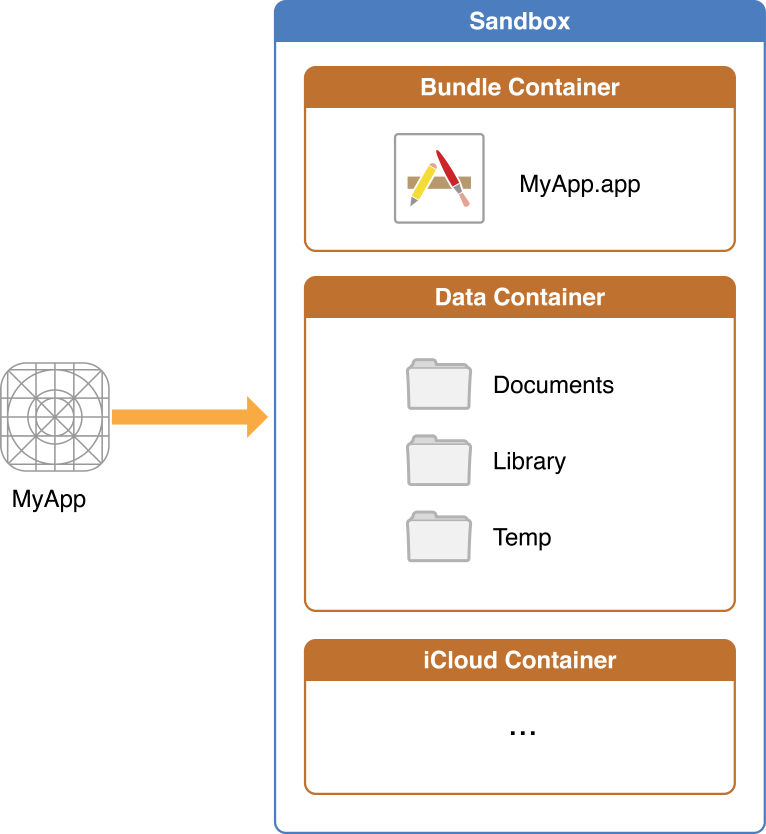
\includegraphics[width=.4\linewidth]{chapter2/ios_about_sandboxing}
    \caption{Arquitectura para proteger los archivos \cite{iosdl}} 
    \label{fig:ch02:sandboxing}
\end{figure}
Si una aplicaci\'on require acceder a información que no es suya, lo puede hacer únicamente usando servicios de iOS. Lo mismo sucede si quiere ejecutar procesos en segundo plano.
Los IDE de iOS construyen las aplicaciones utilizando las técnica ASRL\footnote{La asignación aleatoria del espacio de direcciones (\textit{Address space layout randomization}) es una técnica de seguridad informática involucrada en la prevención contra ataques de desbordamiento de búfer.}, ya que Xcode, el entorno de desarrollo de iOS, compila automáticamente programas de terceros con ASLR activada. De esta forma, se asegura que todas las regiones de memoria son aleatoreas al momento de ejecución \cite{asg}, reduciendo la probabilidad de muchos exploits sofisticados.
\subsection{Controles de privacidad}
iOS ayuda a evitar que las aplicaciones accedan a la información personal de un usuario sin permiso. Las aplicaciones pueden solicitar un permiso solo mientras se est\'a ejecutando o permitirla en cualquier momento. A su vez, los usuarios pueden optar por no permitir este acceso, y pueden cambiar su elección en cualquier momento. Cabe aclarar que una aplicación puede utilizar un recurso sólo si se le ha dado permiso.\\
Además, los usuarios pueden ver qué aplicaciones han permitido acceder a cierta información, así como otorgar o revocar cualquier acceso futuro. Dicha informaci\'on se encuentra en la configuración de privacidad ($Ajustes>>Privacidad$), como se observa en la Figura \ref{fig:ch02:permissions-capture}.\\
\begin{figure}[hbtp]
    \centering
    \begin{subfigure}{0.3\linewidth}
	    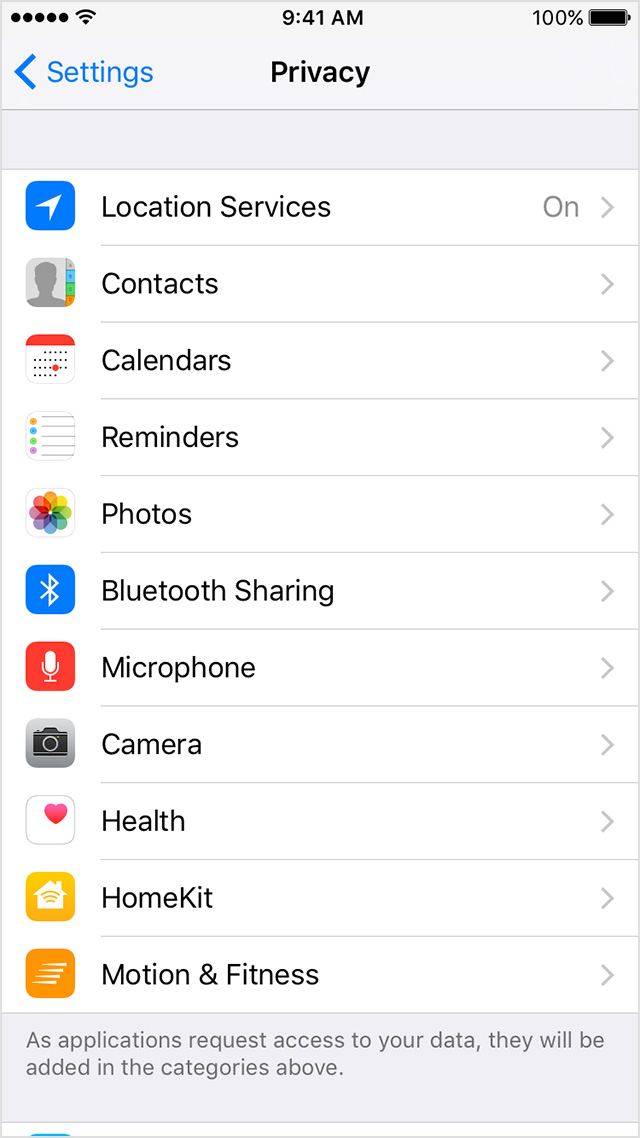
\includegraphics[width=\linewidth]{chapter2/settings-privacy}
	\end{subfigure}
    \begin{subfigure}{0.3\linewidth}
	    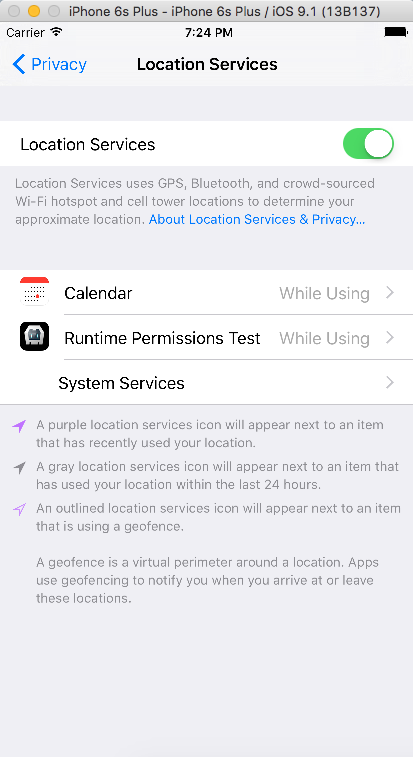
\includegraphics[width=\linewidth]{chapter2/apps-allow-location}
	\end{subfigure}
    \begin{subfigure}{0.3\linewidth}
	    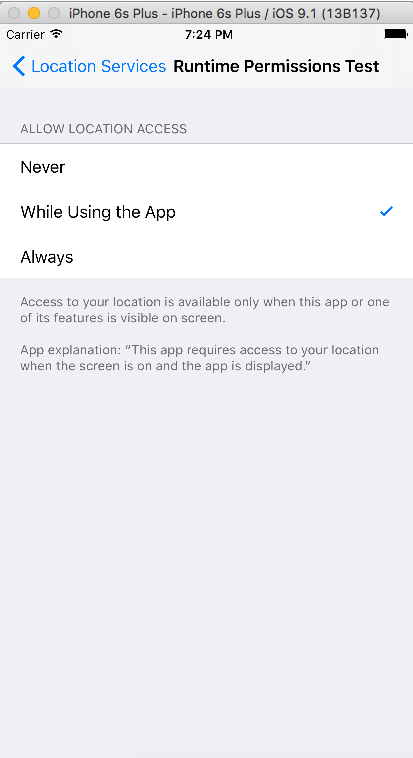
\includegraphics[width=\linewidth]{chapter2/permission-classes}
    \end{subfigure}
    \caption{Control de privacidad de iOS 9.}
	\label{fig:ch02:permissions-capture}
\end{figure}
Los permisos restringen el acceso a:
\begin{multicols}{2}
    \begin{itemize}
        \item Servicios de Localizaci\'on
        \item Contactos
        \item Calendarios
        \item Recordatorios
        \item Fotos
        \item Compartir Bluetooth
        \item Micr\'ofono
        \item C\'amara
        \item Salud
        \item \textit{HomeKit}
        \item Redes Sociales
    \end{itemize} 
\end{multicols}